\documentclass[10pt,a4paper]{amsart}
\usepackage[margin=19mm]{geometry}
\usepackage{amsmath,amssymb,mathtools}
\usepackage[scr=rsfs,cal=euler]{mathalfa}
\usepackage{xfrac}
\usepackage[unicode,hidelinks,bookmarks=false]{hyperref}
\newcommand{\ie}{i.e.\ }
\newcommand{\cf}{cf.\ }
\newcommand{\resp}{respectively\ }
\newcommand{\Subsection}{\subsection}
\providecommand{\nobreakdash}{\nobreak\hbox{-}}
\setlength{\emergencystretch}{2em}
\multlinegap0pt
\usepackage{tikz}
\usepackage{amssymb}
\newtheorem{proposition}{Proposition}
\newtheorem{theorem}{Theorem}
\title{Fourier Levels and Almost Sure Bounds on Higher-Order Derivatives in First-Passage Percolation}
\author{Ivan Matic, Rados Radoicic,, Dan Stefanica}
\date{Source: arXiv:2504.08938v4 (CC BY 4.0)}
\begin{document}
\maketitle

\noindent\emph{Source and licence.} Fourier Levels and Almost Sure Bounds on Higher-Order Derivatives in First-Passage Percolation. Version arXiv:2504.08938v4 (CC BY 4.0), distributed by arXiv under the Creative Commons Attribution 4.0 International licence, http://creativecommons.org/licenses/by/4.0/, as recorded in the arXiv licence metadata for this exact version and shown on the abstract page https://arxiv.org/abs/2504.08938v4. Full licence notice: \texttt{licenses/arxiv-2504.08938-CC-BY-4.0.txt}.\par\smallskip

\noindent\textit{Editorial scope.} Counted unit: the article's theorem thm|lowerBoundS3 (source0.tex lines 1203--1208). The article's complete original proof of it is delivered with it (source0.tex lines 1209--1486, one \texttt{proof} environment of 278 lines). No mathematics is written, repaired or re-derived: the statement and the proof are the article's own lines, in the article's own notation, and no retained line is substituted or re-flowed.  Retained uncounted as the source-local context the proof needs: lines 368--373; lines 1141--1148.  Nothing was omitted from any retained span, so the package carries no omission record.  No retained line contains a citation, so the wrapper carries no bibliography and no bibliography entry.  The retained lines contain the article's own diagram code, which the wrapper typesets with the standard tikz packages; no image file is delivered and the package declares no asset dependency.  Editorial formatting only, in addition: an AMS \texttt{amsart} preamble that restates the article's own declarations and macros used by the retained lines, namely the environments \texttt{proposition}, \texttt{theorem} on separate counters, together with the standard packages those lines need.  The retained environments print in this document as Proposition 1, Theorem 1 in order of appearance, whereas the article prints the same items with the numbering of its own full document.  The complete native source of the article as distributed in the arXiv e-print for this exact version is bundled unchanged as \texttt{sources/176410/source0.tex}.
\begin{proposition}\label{thm|forComputer} The following two propositions hold for every $\omega\in\Omega$.
\begin{enumerate}
\item[(a)] If $\sigma_j^a(\omega)\in E_j^C$, then $f(\sigma_j^b(\omega))=f(\sigma_j^a(\omega))$;
\item[(b)] If $\sigma_j^b(\omega)\in \hat E_j$, then $f(\sigma_j^b(\omega))=f(\sigma_j^a(\omega))+(b-a)$.
\end{enumerate}
\end{proposition} 

\begin{proposition}\label{thm|lowerBoundS3DSwitch} 
Assume that $S=\{k,l,m\}$ and that for fixed environment $\omega$, $k$ is a direction switching edge with respect to 
$(l,m)$.
The following inequality must hold
\begin{eqnarray} 
\partial_Sf(\omega)&\geq&3a-b.\label{eqn|BoundS3DirectionSwitch}
\end{eqnarray}
\end{proposition}

\begin{theorem}\label{thm|lowerBoundS3}
Let $S\subseteq W$ be a subset with three elements. The first passage percolation time $f$ satisfies the following inequality for every $\omega\in\Omega$
\begin{eqnarray}
\partial_Sf(\omega)&\geq& -(b-a). \label{eqn|lowerBoundS3}
\end{eqnarray}
\end{theorem}

\begin{proof} Let $S=\{k,l,m\}$. Due to Proposition \ref{thm|lowerBoundS3DSwitch} and $3a-b> -(b-a)$, we may assume that none of the edges is direction-switching with respect to the other two. 

We will first prove the following implication
\begin{eqnarray}
\sigma^{(a,a,b)}(\omega)\not\in E_k\cap E_l\cap \hat E_m^C&\Longrightarrow& \partial_Sf(\omega)\geq -(b-a)
\label{eqn|lowerBoundS3ImplicationMain}
\end{eqnarray}
The result \eqref{eqn|lowerBoundS3ImplicationMain} will follow from the following two
\begin{eqnarray}
\sigma^{(a,a,b)}(\omega)\in E_k^C &\Longrightarrow& \partial_Sf(\omega)\geq -(b-a),\label{eqn|lowerBoundS3ImplicationA}\\
\sigma^{(a,a,b)}(\omega)\in \hat E_m &\Longrightarrow& \partial_Sf(\omega)\geq -(b-a).\label{eqn|lowerBoundS3ImplicationB}
\end{eqnarray}
The first step in proving \eqref{eqn|lowerBoundS3ImplicationA} is to express the derivative $\partial_Sf(\omega)$ 
as 
\begin{eqnarray}
\partial_Sf(\omega)&=& \left(f(\sigma^{(b,b,b)}(\omega))-f(\sigma^{(b,b,a)}(\omega))\right) \label{eqn|lbS3ImpADer01}\\
&& +\left(f(\sigma^{(b,a,a)}(\omega))-
f(\sigma^{(a,a,a)}(\omega))\right) \label{eqn|lbS3ImpADer02}\\
&&-\left(f(\sigma^{(b,a,b)}(\omega))-f(\sigma^{(a,a,b)}(\omega))\right) \label{eqn|lbS3ImpADer03}\\
&&-\left(f(\sigma^{(a,b,b)}(\omega))-f(\sigma^{(a,b,a)}(\omega))
\right). \label{eqn|lbS3ImpADer04}
\end{eqnarray}
Assume that $\sigma^{(a,a,b)}(\omega)\in E_k^C$. Proposition \ref{thm|forComputer} (a) implies that the term \eqref{eqn|lbS3ImpADer03} 
is equal to $0$. The terms \eqref{eqn|lbS3ImpADer01} and \eqref{eqn|lbS3ImpADer02} are non-negative, and the negative term \eqref{eqn|lbS3ImpADer04} is bounded below
by $-(b-a)$, which proves \eqref{eqn|lowerBoundS3ImplicationA}.
In order to prove \eqref{eqn|lowerBoundS3ImplicationB}, we start by expressing $\partial_Sf(\omega)$ as 
\begin{eqnarray}
\partial_Sf(\omega)&=& \left(f(\sigma^{(b,b,b)}(\omega))-f(\sigma^{(b,b,a)}(\omega))\right) \label{eqn|lbS3ImpBDer01}\\
&& +\left(f(\sigma^{(a,a,b)}(\omega))-
f(\sigma^{(a,a,a)}(\omega))\right) \label{eqn|lbS3ImpBDer02}\\
&&-\left(f(\sigma^{(b,a,b)}(\omega))-f(\sigma^{(b,a,a)}(\omega))\right) \label{eqn|lbS3ImpBDer03}\\
&&-\left(f(\sigma^{(a,b,b)}(\omega))-f(\sigma^{(a,b,a)}(\omega))
\right). \label{eqn|lbS3ImpBDer04}
\end{eqnarray}
Assume that $\sigma^{(a,a,b)}(\omega)\in \hat E_m$. Proposition \ref{thm|forComputer} (b) implies that the term \eqref{eqn|lbS3ImpBDer02} is equal to $(b-a)$. The term 
\eqref{eqn|lbS3ImpBDer01} is non-negative. The terms \eqref{eqn|lbS3ImpBDer03} and \eqref{eqn|lbS3ImpBDer04} are negative but bounded below by $-(b-a)$. Therefore, $\partial_Sf(\omega)$ is bounded below by $(b-a)-2(b-a)=-(b-a)$. This completes the proof of \eqref{eqn|lowerBoundS3ImplicationB}. 

We proved \eqref{eqn|lowerBoundS3ImplicationMain} which states that the inequality $\partial_S f(\omega)\geq -(b-a)$ is satisfied unless 
$\sigma^{(a,a,b)}(\omega)$ is an element of $E_k\cap E_l\cap \hat E_m^C$. The analogous statements hold for $\sigma^{(a,b,a)}(\omega)$ and $\sigma^{(b,a,a)}(\omega)$. Hence, the required bound \eqref{eqn|lowerBoundS3} is proved unless all of the following three inclusions are satisfied
\begin{eqnarray}
\sigma^{(a,a,b)}(\omega)&\in& E_k\cap E_l\cap \hat E_m^C, \label{eqn|bS3Inclaab}\\
\sigma^{(a,b,a)}(\omega)&\in& E_k\cap \hat E_l^C\cap E_m,\quad\mbox{and} \label{eqn|bS3Inclaba}\\
\sigma^{(b,a,a)}(\omega)&\in& \hat E_k^C\cap E_l\cap E_m. \label{eqn|bS3Inclbaa}
\end{eqnarray}
Hence, it suffices to prove $\partial_Sf\geq -(b-a)$ under the conditions \eqref{eqn|bS3Inclaab}, \eqref{eqn|bS3Inclaba}, and \eqref{eqn|bS3Inclbaa}.
Due to $\sigma^{(a,a,b)}(\omega)\in \hat E_m^C$, there exists a geodesic on $\sigma^{(a,a,b)}(\omega)$ that does not contain the edge $m$. Let us fix one such geodesic and denote it by $\gamma_{kl}$. Since $\sigma^{(a,a,b)}(\omega)\in E_k\cap E_l$, the geodesic $\gamma_{kl}$ must contain both edges $k$ and $l$. We define the geodesics $\gamma_{lm}$ and $\gamma_{km}$ in analogous ways. Once the paths $\gamma_{kl}$, $\gamma_{lm}$, and $\gamma_{km}$ are fixed, we define the relation $\prec$ on $\{k,l,m\}$. We will write $k\prec l$ if on the path $\gamma_{kl}$ the edge $k$ appears before the edge $l$ when moving from the source to the sink. There are two cases: 
\begin{itemize}
\item Case 1: The relation $\prec$ does not have a minimum;
\item Case 2: The relation $\prec$ has a minimum.
\end{itemize}

\noindent {\bf Case 1.} This case is easier to consider. We may assume that $k\prec l$, $l\prec m$, and $m\prec k$. 

 \begin{figure}[t]
 \centering
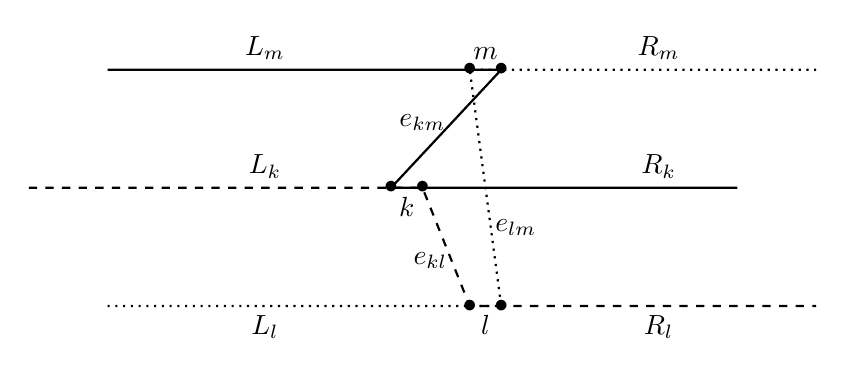
\begin{tikzpicture}
\draw[thick] (1,3.5) -- (6,3.5) -- (4.6,2) -- (9,2);
\draw[thick,dashed] (0,2) -- (5,2) -- (5.6,0.5) -- (10,0.5); 
\draw[thick,dotted] (1,0.5) -- (6,0.5) -- (5.6,3.5) -- (10,3.5); 
\node at (5.6,3.5) {$\bullet$};
\node at (6,3.5) {$\bullet$};
\node[above] at (5.8,3.5) {$m$}; 
\node at (6,0.5) {$\bullet$};
\node at (5.6,0.5) {$\bullet$};
\node[below] at (5.8,0.5) {$l$}; 
\node at (4.6,2) {$\bullet$};
\node at (5,2) {$\bullet$};
\node[below] at (4.8,2) {$k$}; 
\node[above] at (3,3.5) {$L_m$};
\node[above] at (8,3.5) {$R_m$};
\node[above] at (3,2) {$L_k$};
\node[above] at (8,2) {$R_k$};
\node[below] at (3,0.5) {$L_l$};
\node[below] at (8,0.5) {$R_l$};
\node[above] at (5.0,2.60) {$e_{km}$};
\node[below] at (5.1,1.30) {$e_{kl}$};
\node[right] at (5.8,1.5) {$e_{lm}$};
\end{tikzpicture}
\caption{Case in which $\prec$ has no minimum.}
\label{fig|LowerBound3NoMin}
\end{figure}

As we mentioned earlier, the Proposition \ref{thm|lowerBoundS3DSwitch} allowed us to assume that the directions of the flow over the edges $k$, $l$, and $m$ is the same on the environments 
$\sigma^{(a,a,b)}(\omega)$, $\sigma^{(a,b,a)}(\omega)$, and $\sigma^{(b,a,a)}(\omega)$.  

Let us denote by $e_{kl}$ the total passage time between the edges $k$ and $l$ on the geodesic $\gamma_{kl}$. We define $e_{km}$ and $e_{lm}$ in analogous way. 
Let us denote by $L_k$ the total passage time on the geodesic $\gamma_{kl}$ before the edge $k$. Let $R_l$ be the total passage time on the geodesic $\gamma_{kl}$ after the edge $l$. 
The numbers $L_m$, $L_l$, $R_k$, and $R_m$ are defined in similar ways. Let us emphasize that none of the previously defined passage times includes the edges $k$, $m$, and $l$. 

Since the paths $\gamma_{kl}$, $\gamma_{lm}$, and $\gamma_{km}$ are fixed, the quantities $e_{\cdot\cdot}$, $R_{\cdot}$, and $L_{\cdot}$ that we defined 
above are the same on the environments $\sigma^{\overrightarrow{\theta}}(\omega)$ for all eight choices $\overrightarrow \theta \in\{a,b\}^3$.
We will now prove the following identities
\begin{eqnarray}
f(\sigma^{(a,a,b)}(\omega))&=&L_k+e_{kl}+R_l+2a,\label{eqn|lbS3Case101}\\
f(\sigma^{(a,b,a)}(\omega))&=&L_m+e_{km}+R_k+2a,\label{eqn|lbS3Case102}\\
f(\sigma^{(b,a,a)}(\omega))&\geq& f(\sigma^{(a,a,a)}(\omega)),\label{eqn|lbS3Case103}\\
f(\sigma^{(b,b,b)}(\omega))&\geq& f(\sigma^{(b,b,a)}(\omega)),\label{eqn|lbS3Case104}\\
f(\sigma^{(b,a,b)}(\omega))&\leq& L_l+a+R_l,\label{eqn|lbS3Case105}\\
f(\sigma^{(a,b,b)}(\omega))&\leq& L_k+a+R_k.\label{eqn|lbS3Case106}
\end{eqnarray}
The equalities \eqref{eqn|lbS3Case101} and \eqref{eqn|lbS3Case102} are due to the definitions of $\gamma_{kl}$ and $\gamma_{km}$. The inequalities \eqref{eqn|lbS3Case103} and 
\eqref{eqn|lbS3Case104} are the consequences of monotonicity. 


Let us prove \eqref{eqn|lbS3Case105}. On the environment $\sigma^{(b,a,b)}(\omega)$, we
will construct a path $\delta$ such that 
\begin{eqnarray*}T(\delta, \sigma^{(b,a,b)}(\omega)) &=& L_l+a+R_l.
\end{eqnarray*}
Let us identify the section of the path $\gamma_{lm}$ before the edge $l$ and call it $\delta_1$. 
It has the passage time $L_l$. Let us consider the section of the path $\gamma_{kl}$ after the edge $l$. 
This section will be called $\delta_2$. Its passage time is $R_l$. 
Now we define $\delta=\delta_1\cup\{l\}\cup \delta_2$. This path $\delta$ connects the source and the sink. Its passage time is $L_l+a+R_l$, hence \eqref{eqn|lbS3Case105} must hold. 

The inequality \eqref{eqn|lbS3Case106} is proved in a similar way.

From \eqref{eqn|lbS3Case101}--\eqref{eqn|lbS3Case106} we obtain 
\begin{eqnarray}
\partial_Sf(\omega)&\geq& (L_k+e_{kl}+R_l+2a) + (L_m+e_{km}+R_k+2a) \nonumber\\
&&-(L_l+a+R_l)-(L_k+a+R_k) \nonumber \\
&=& e_{kl}   + L_m+e_{km}+ 2a 
-L_l. \label{eqn|lbS3Case107}
\end{eqnarray}
Let us consider the geodesic $\gamma_{lm}$ on the environment $\sigma^{(b,a,a)}(\omega)$. Let us consider $\hat \xi$ 
that consists of the union of the left part of $\gamma_{km}$ and the right part of $\gamma_{lm}$. 
The path $\xi=\hat\xi\cup\{m\}$ is a path between the source and the sink whose passage 
time is $L_m+a+R_m$.  Hence, we found a path between the source and the 
sink whose passage time is equal to $L_m+a+R_m$. Since $\gamma_{lm}$ is a geodesic with passage time 
$L_l+e_{lm}+R_m+2a$, we obtain
$L_m+a+R_m \geq L_l+e_{lm}+R_m+2a$. The last inequality is equivalent to $L_m-L_l\geq e_{lm}+a$. The inequality \eqref{eqn|lbS3Case107} turns into 
$\partial_Sf(\omega)\geq e_{kl}+e_{km}+e_{lm}+3a\geq 3a>-(b-a)$. We have completed the proof in Case 1. 

 
\noindent{\bf Case 2.} We may assume that $k$ is the minimum, i.e. $k\prec l$ and $k\prec m$. Without loss of generality, we may assume that $l\prec m$. 

 \begin{figure}[t]
 \centering
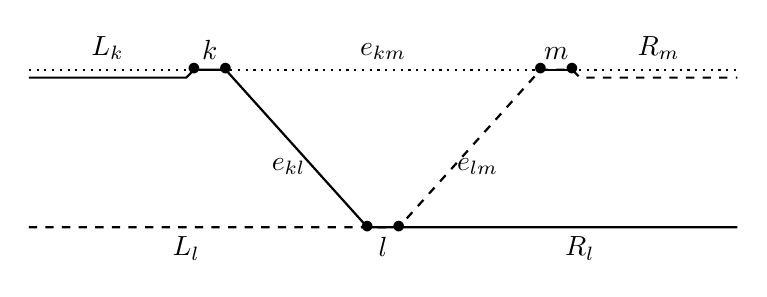
\begin{tikzpicture}
\draw[thick,dotted] (0.5,2.5) -- (3,2.5) -- (7,2.5) -- (9.5,2.5);
\draw[thick,dashed] (0.5,0.5) -- (5.2,0.5) -- (7,2.5) -- (7.4,2.5) -- (7.5,2.4) -- (9.5,2.4);
\draw[thick] (0.5,2.4) -- (2.5,2.4) --(2.6,2.5) --(3,2.5) -- (4.8,0.5) -- (9.5,0.5);
\draw[thick] (7.0,2.5) -- (7.4,2.5);
\draw[thick] (4.8,0.5) -- (5.2,0.5);
\node at (3,2.5) {$\bullet$};
\node at (2.6,2.5) {$\bullet$};
\node[above] at (2.8,2.5) {$k$};
\node at (7,2.5) {$\bullet$};
\node at (7.4,2.5) {$\bullet$};
\node[above] at (7.2,2.5) {$m$};
\node at (4.8,0.5) {$\bullet$};
\node at (5.2,0.5) {$\bullet$};
\node[below] at (5,0.5) {$l$};
\node[above] at (1.5,2.5) {$L_k$};
\node[above] at (8.5,2.5) {$R_m$};
\node[above] at (5,2.5) {$e_{km}$};
\node[below] at (3.8,1.5) {$e_{kl}$};
\node[below] at (6.2,1.5) {$e_{lm}$};
\node[below] at (2.5,0.5) {$L_l$};
\node[below] at (7.5,0.5) {$R_l$};
\end{tikzpicture}
\caption{Case in which $k\prec l\prec m$.}
\label{fig|lowerBound3TriangleNoAlLRA}
\end{figure}

 Figure \ref{fig|lowerBound3TriangleNoAlLRA} corresponds to the situation in which $k\prec l\prec m$. 
 
The sections of the paths $\gamma_{kl}$ and $\gamma_{km}$ before the edge $k$ must have equal passage times. Let us denote by $L_k$ the common passage time of these sections. We may modify one of the paths $\gamma_{kl}$ and $\gamma_{km}$ in such a way that the sections before $k$ actually coincide. In a similar way, the passage times after the edge $m$ on the paths $\gamma_{km}$ and $\gamma_{lm}$ are equal. We will denote these passage times by $R_m$. We define $L_l$ as the passage time over the path $\gamma_{lm}$ before the edge $l$; $R_l$ the passage time over $\gamma_{kl}$ after $l$. We define $e_{kl}$, $e_{lm}$, and $e_{km}$ as passage times over the open intervals $(k,l)$, $(l,m)$, and $(k,m)$ on the paths 
$\gamma_{kl}$, $\gamma_{lm}$, and $\gamma_{km}$, respectively. Let us define the real number $\theta$ in such a way that $e_{km} =e_{kl}+e_{lm}+a+\theta$, i.e.
\begin{eqnarray} \theta &=&
e_{km} -e_{kl}-e_{lm}-a
 .\label{eqn|lbS3Case1Theta}\end{eqnarray} 
We don't know whether $\theta$ is positive or negative. However, we will
be able to prove that $\theta$ satisfies the inequality 
\begin{eqnarray}\theta\leq b-a,\label{eqn|InequalityTheta}\end{eqnarray}
which is sufficient for our needs. 
On the environment $\sigma^{(a,b,a)}(\omega)$, the minimal passage time is over the path $\gamma_{km}$. This passage time is $L_k+e_{km}+R_m+2a$. 
Consider the path in which the segment $(k,m)$ is replaced with $(k,l)\cup \{l\}\cup (l,m)$ (i.e., the section of $\gamma_{kl}$ between $k$ and $l$, the edge $l$, and 
the section of $\gamma_{lm}$ between $l$ and $m$). The passage time of this path is 
$L_k+e_{kl}+e_{lm}+R_m+2a+b$. The latter number is larger than the former, hence 
\[L_k+e_{kl}+e_{lm}+R_m+2a+b>L_k+e_{km}+R_m+2a,\]
which, together with \eqref{eqn|lbS3Case1Theta}, implies \eqref{eqn|InequalityTheta}.

Let us define the real numbers $\theta_L$ and $\theta_R$ with the following two identities
\begin{eqnarray}
L_l&=&L_k+e_{kl}+a+\theta_L,\label{eqn|lbS3Case1ThetaL}\\
R_l&=&R_m+e_{lm}+a+\theta_R.\label{eqn|lbS3Case1ThetaR}
\end{eqnarray}
The numbers $\theta_L$ and $\theta_R$ must belong to the interval $(0,b-a]$. Let us prove that $\theta_L\in(0,b-a]$. We need to prove $\theta_L>0$ and $\theta_L\leq b-a$. 

In order to prove
$\theta_L>0$, we start by observing that on $\sigma^{(a,a,b)}(\omega)$, every geodesic must go through $k$. The path $\gamma_{kl}$ is a geodesic. 
Let us take the section of this geodesic before the edge $l$ and replace it with the corresponding section of $\gamma_{lm}$.
We obtain a path that is not a geodesic because it omits $k$, while \eqref{eqn|bS3Inclaab} claims that every geodesic on $\sigma^{(a,a,b)}(\omega)$ must contain $k$. The change of passage time must satisfy \begin{eqnarray}0&<&L_l-L_k-a-e_{kl}= \theta_L. \label{eqn|equivalentIneqThetaL}\end{eqnarray}
 

Let us now prove that $\theta_L\leq b-a$. Consider the environment $\sigma^{(b,a,a)}(\omega)$. The path $\gamma_{lm}$ is a geodesic. Let us denote by $\gamma_{kl}^-$ the section of $\gamma_{kl}$ before the edge $l$. Let $\gamma_{lm}^+$ be the section of $\gamma_{lm}$ after the edge $l$. The path $\gamma_{kl}^-\cup\{l\}\cup \gamma_{lm}^+$ is a path from the source to the sink that has passage time $L_k+e_{kl}+e_{lm}+R_m+2a+b$. 
The passage time over the geodesic $\gamma_{lm}$ is 
$L_l+e_{lm}+R_m+2a$. From 
\begin{eqnarray*}L_l+e_{lm}+R_m+2a&\leq &L_k+e_{kl}+e_{lm}+R_m+2a+b,
\end{eqnarray*}
we obtain  $L_l  \leq L_k+e_{kl} +  b$. The last inequality and  \eqref{eqn|lbS3Case1ThetaL} imply $\theta_L\leq (b-a)$.
 
In an analogous way we prove that $\theta_R\in (0,b-a]$. 

We can now update our picture. Figure \ref{fig|lowerBound3TriangleNoAlLRAUpdated} shows the geodesics in which the labels $L_l$, $e_{km}$, and $R_L$ are replaced with their equivalent values involving $\theta$, $\theta_L$, and $\theta_R$.

 \begin{figure}[t]
 \centering
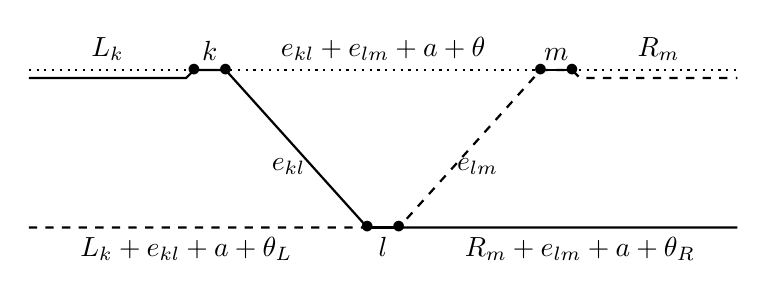
\begin{tikzpicture}
\draw[thick,dotted] (0.5,2.5) -- (3,2.5) -- (7,2.5) -- (9.5,2.5);
\draw[thick,dashed] (0.5,0.5) -- (5.2,0.5) -- (7,2.5) -- (7.4,2.5) -- (7.5,2.4) -- (9.5,2.4);
\draw[thick] (0.5,2.4) -- (2.5,2.4) --(2.6,2.5) --(3,2.5) -- (4.8,0.5) -- (9.5,0.5);
\draw[thick] (7.0,2.5) -- (7.4,2.5);
\draw[thick] (4.8,0.5) -- (5.2,0.5);
\node at (3,2.5) {$\bullet$};
\node at (2.6,2.5) {$\bullet$};
\node[above] at (2.8,2.5) {$k$};
\node at (7,2.5) {$\bullet$};
\node at (7.4,2.5) {$\bullet$};
\node[above] at (7.2,2.5) {$m$};
\node at (4.8,0.5) {$\bullet$};
\node at (5.2,0.5) {$\bullet$};
\node[below] at (5,0.5) {$l$};
\node[above] at (1.5,2.5) {$L_k$};
\node[above] at (8.5,2.5) {$R_m$};
\node[above] at (5,2.5) {$e_{kl}+e_{lm}+a+\theta$};
\node[below] at (3.8,1.5) {$e_{kl}$};
\node[below] at (6.2,1.5) {$e_{lm}$};
\node[below] at (2.5,0.5) {$L_k+e_{kl}+a+\theta_L$};
\node[below] at (7.5,0.5) {$R_m+e_{lm}+a+\theta_R$};
\end{tikzpicture}
\caption{The labels $L_l$, $e_{km}$, and $R_L$ are replaced with their equivalent values involving $\theta$, $\theta_L$, and $\theta_R$.}
\label{fig|lowerBound3TriangleNoAlLRAUpdated}
\end{figure}

 Since $\gamma_{kl}$, $\gamma_{lm}$, and $\gamma_{km}$ are geodesics on $\sigma^{(a,a,b)}(\omega)$, $\sigma^{(b,a,a)}(\omega)$, and $\sigma^{(a,b,a)}(\omega)$, respectively, we obtain 
\begin{eqnarray}
f(\sigma^{(a,a,b)}(\omega))&=&L_k+R_m+e_{kl}+e_{lm}+3a+\theta_R,\label{eqn|lbS3f01}\\
f(\sigma^{(a,b,a)}(\omega))&=&L_k+R_m+e_{kl}+e_{lm}+3a+\theta,\label{eqn|lbS3f02}\\
f(\sigma^{(b,a,a)}(\omega))&=&L_k+R_m+e_{kl}+e_{lm}+3a+\theta_L.\label{eqn|lbS3f03}
\end{eqnarray}
Due to monotonicity we have 
\begin{eqnarray}
f(\sigma^{(b,b,b)}(\omega))&\geq& f(\sigma^{(a,b,b)}(\omega)). \label{eqn|lbS3f04}
\end{eqnarray}
Let us consider the environment $\sigma^{(b,a,b)}(\omega)$. We will construct a path $\zeta$ that has a low passage time and that will provide a useful upper bound for $f(\sigma^{(b,a,b)}(\omega))$.   
Let $\gamma_{lm}^-$ be the section of $\gamma_{lm}$ before $l$. Let $\gamma_{kl}^+$ be the section of $\gamma_{kl}$ after $l$. 
Define $\zeta=\gamma_{lm}^-\cup \{l\}\cup \gamma_{kl}^+$. The passage time over $\zeta$ is equal to $L_k+$ $e_{kl}+$ $\theta_L+$ $R_m+$ $e_{lm}+$ $\theta_R+$ $3a$. 
The passage time over $\zeta$ is greater than or equal to the minimal passage time, hence
\begin{eqnarray}
f(\sigma^{(b,a,b)}(\omega))&\leq&L_k+R_m+e_{kl}+e_{lm}+3a+\theta_L+\theta_R. \label{eqn|lbS3f05}
\end{eqnarray}
The minimal passage time $f(\sigma^{(b,b,a)}(\omega))$ is smaller than or equal to the minimum 
of the passage times over the paths $\gamma_{lm}$ and $\gamma_{km}$, hence
\begin{eqnarray}
f(\sigma^{(b,b,a)}(\omega))&\leq& L_k+R_m+e_{kl} +e_{lm}+2a+b+\min\{\theta_L,\theta \}.\label{eqn|lbS3f06} 
\end{eqnarray}
Finally, let us consider the environment $\sigma^{(a,a,a)}(\omega)$. By considering the passage time over the path $\gamma_{km}$, we obtain 
\begin{eqnarray}
f(\sigma^{(a,a,a)}(\omega))&\leq& L_k+R_m+e_{kl}+e_{lm}+3a+\theta.\label{eqn|lbS3f0701}
\end{eqnarray}
Let us construct an alternative path $\gamma'$ on the environment $\sigma^{(a,a,a)}(\omega)$. We replace the section $(k,m)$ with the sections $(k,l)$ and $(l,m)$ of the paths $\gamma_{kl}$ and $\gamma_{lm}$. We must also add the edge $l$ in order for $\gamma'$ to connect source to the sink. The passage time over $\gamma'$ is $L_k+R_m+e_{kl}+e_{lm}+3a$, hence 
\begin{eqnarray}
f(\sigma^{(a,a,a)}(\omega))&\leq& L_k+R_m+e_{kl}+e_{lm}+3a.\label{eqn|lbS3f0702}
\end{eqnarray}
The inequalities \eqref{eqn|lbS3f0701} and \eqref{eqn|lbS3f0702} imply 
\begin{eqnarray}
f(\sigma^{(a,a,a)}(\omega))&\leq& L_k+R_m+e_{kl}+e_{lm}+3a+\min\{\theta,0\}. \label{eqn|lbS3f07}
\end{eqnarray}
We now use \eqref{eqn|lbS3f01}--\eqref{eqn|lbS3f06} and \eqref{eqn|lbS3f07} to find the lower bound on $\partial_Sf(\omega)$. Observe that $L_k+R_m+e_{kl}+e_{lm}$ appears equally many times with sign $+$ as with sign $-$. We can ignore these terms as they cancel out in the evaluation of $\partial_Sf(\omega)$. Hence, 
\begin{eqnarray}
\partial_Sf(\omega)&\geq&   a    -b+\theta -\min\{\theta_L,\theta\} -\min\{\theta,0\}. \label{eqn|lbS3AlmostDone}
\end{eqnarray}
Define
$F(\theta,\theta_L)=\theta- \min\{\theta_L,\theta\}-\min\{\theta,0\}$. It suffices to prove that $F(\theta,\theta_L)\geq 0$. 
There are two cases: $\theta\geq 0$ and $\theta<0$. If $\theta\geq 0$, then $\min\{\theta,0\}=0$ and $F(\theta,\theta_L)=\theta-\min\{\theta_L,\theta\}\geq 0$. 
If $\theta <0$, then from $\theta_L>0$ we have $\min\{\theta,\theta_L\}=\theta$, and  
$F(\theta,\theta_L)=\theta-\theta-\theta=-\theta>0$. This completes the proof of Case 2, which was the only remaining case that we needed to consider.
\end{proof}

\end{document}
